\section{Venneliste}
I vennelistecontrolleren er der implementeret en venneliste, som indeholder brugere, der følges. For at app'en kan hente venner som brugeren følger, sendes brugerens medlemsID til databasen. Et php-script benytter medlemsid i en SQL-kommando, der tilgår tabellen for vennerelationer, som returnerer \textit{ven$\_$medlemsid} med tilhørende navn for de brugere, der følges. 
Dette modtages i app'en som et JSON-objekt, hvorfra et JSON-array hentes og ligges i et array. Dette kan ses af udklippet i \autoref{fig:vennerKode}.  

\begin{figure} [H]
\centering
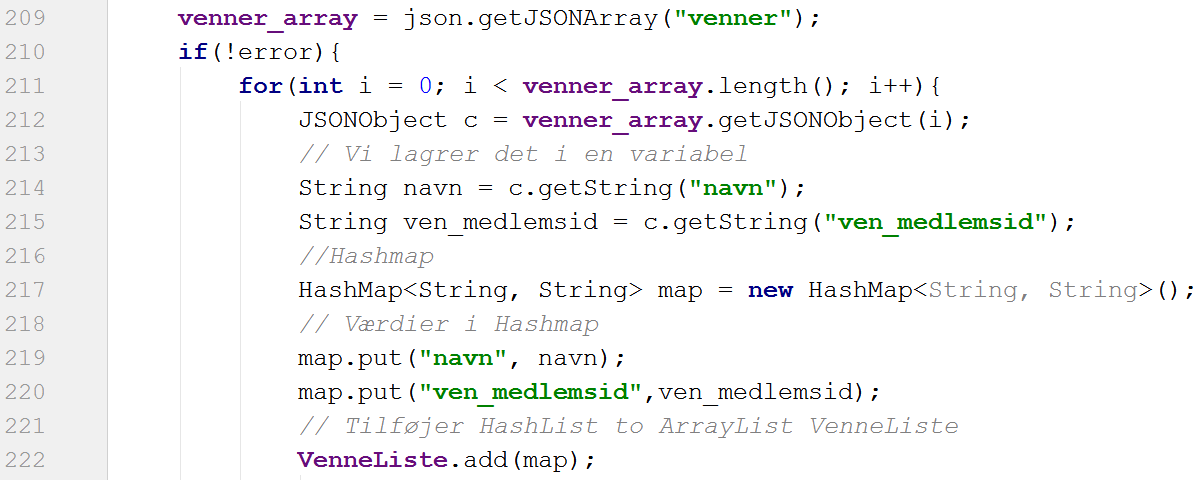
\includegraphics[width=1\textwidth]{figures/imple/vennerKode}
\caption{Udpluk af koden for venneliste. Koden viser et udpluk af, hvordan venners navn og medlemsid gemmes i arraylisten, VenneListe.}
\label{fig:vennerKode}
\end{figure}

\noindent
Af koden i figuren er der opsat en for-loop, hvori JSON-objekter hentes fra alle placeringerne i et array kaldet \textit{venner$\_$array}. Hvert af disse objekter repræsenterer én af brugerens venner, hvor værdier for \textit{navn} og \textit{ven$\_$medlemsid} er hentet. 
Af for-loopen ses det, at objekterne gemmes i et nyt array af navnet VenneListe, som senere benyttes til at opstille vennerne i ListView for grænsefladen. Grundet bruget af HashMap til at håndtere \textit{navn} og \textit{ven$\_$medlemsid}, har det været nødvendigt at håndtere medlemsid som en string. Dette skyldes, at ved instansiering af Hashmappet defineres inputstyperne som string, idet navnet er af typen string. 

Der er i app'en ligeledes mulighed for at tilføje og fjerne brugere fra vennelisten. Muligheden for at tilføje en bruger til vennelisten er implementeret ved at benytte SQL-kommandoen, der ses af \autoref{fig:opretVenKode}.

\begin{figure} [H]
\centering
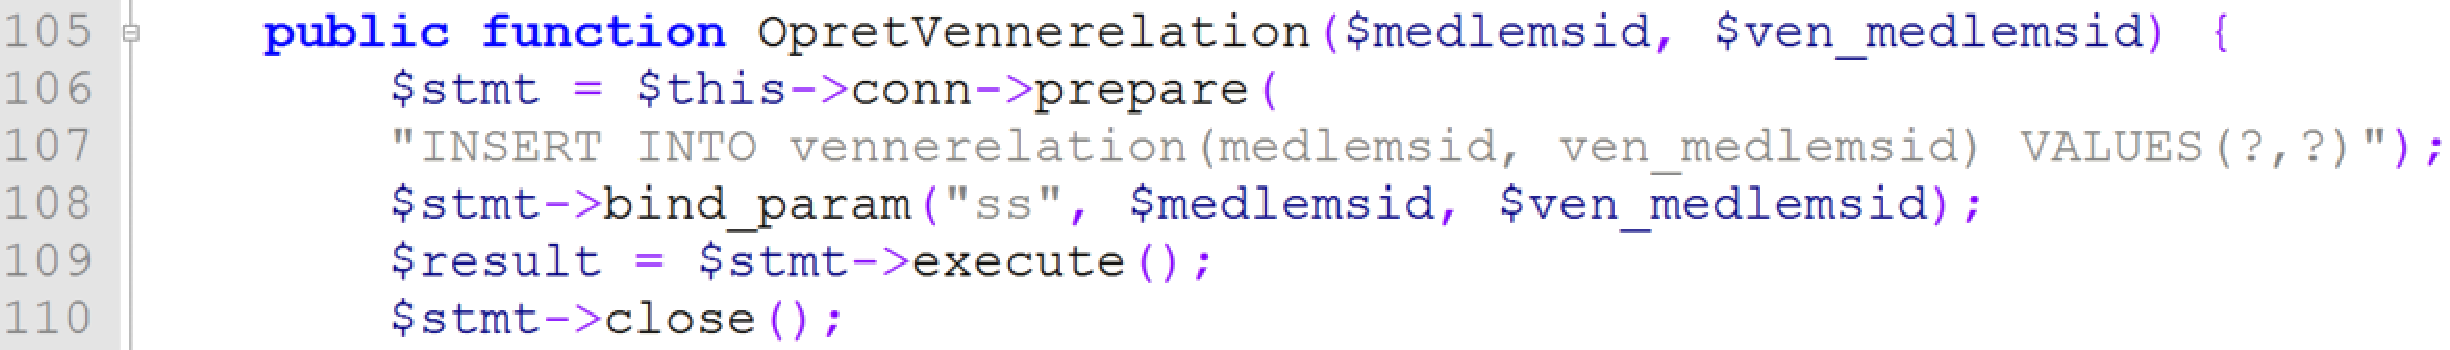
\includegraphics[width=1\textwidth]{figures/imple/opretVenKode}
\caption{SQL-kommando for tilføj bruger til venneliste.}
\label{fig:opretVenKode}
\end{figure}

\noindent
I ovenstående kode ses det, at medlemsid og ven$\_$medlemsid indsættes i tabellen, Vennerelation, hvorved der dannes en vennerelation. Fjernes en bruger fra vennelisten, anvendes SQL-kommandoen, der fremgår af \autoref{fig:fjernVenKode}. Dertil er forskellen fra at oprette en vennerelation, at SQL-kommandoen anvender delete, og dermed fjerner vennerelationen fra tabellen i databasen. Hertil fjernes relationen kun, hvis både medlemsID for bruger og ven indgår. 

\begin{figure} [H]
\centering
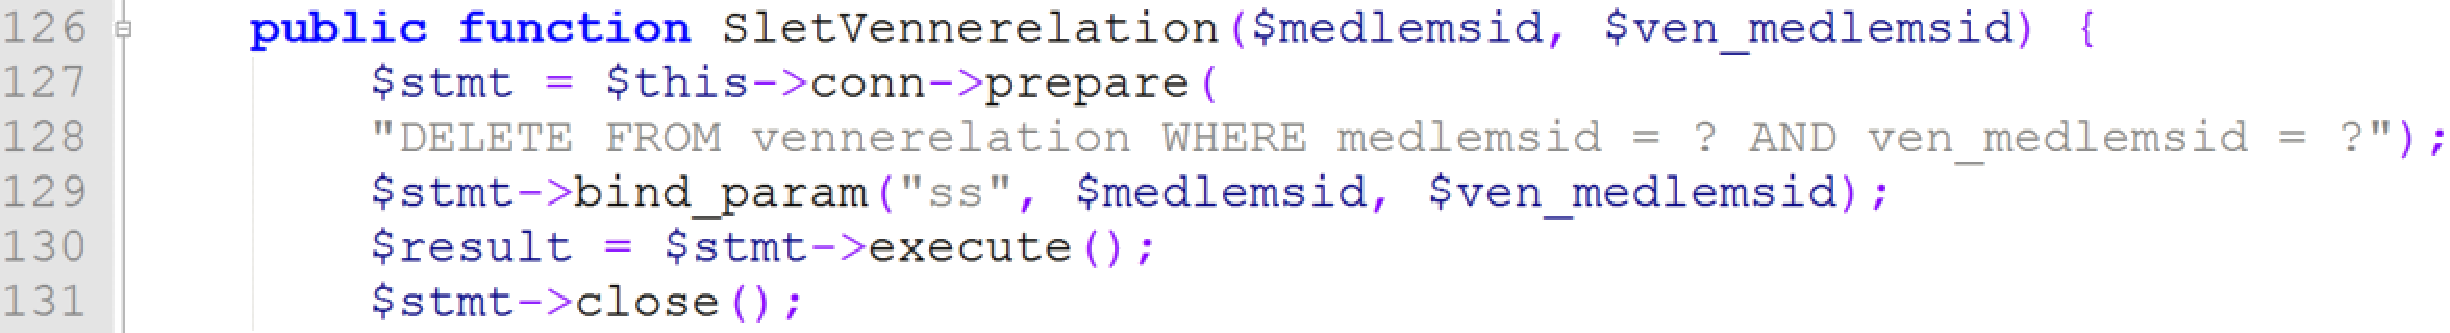
\includegraphics[width=1\textwidth]{figures/imple/fjernVenKode}
\caption{SQL-kommando for fjern bruger til venneliste.}
\label{fig:fjernVenKode}
\end{figure}

